\chapter{Geometry}

\section{Voronoi - Delanauy dual}

\centerline{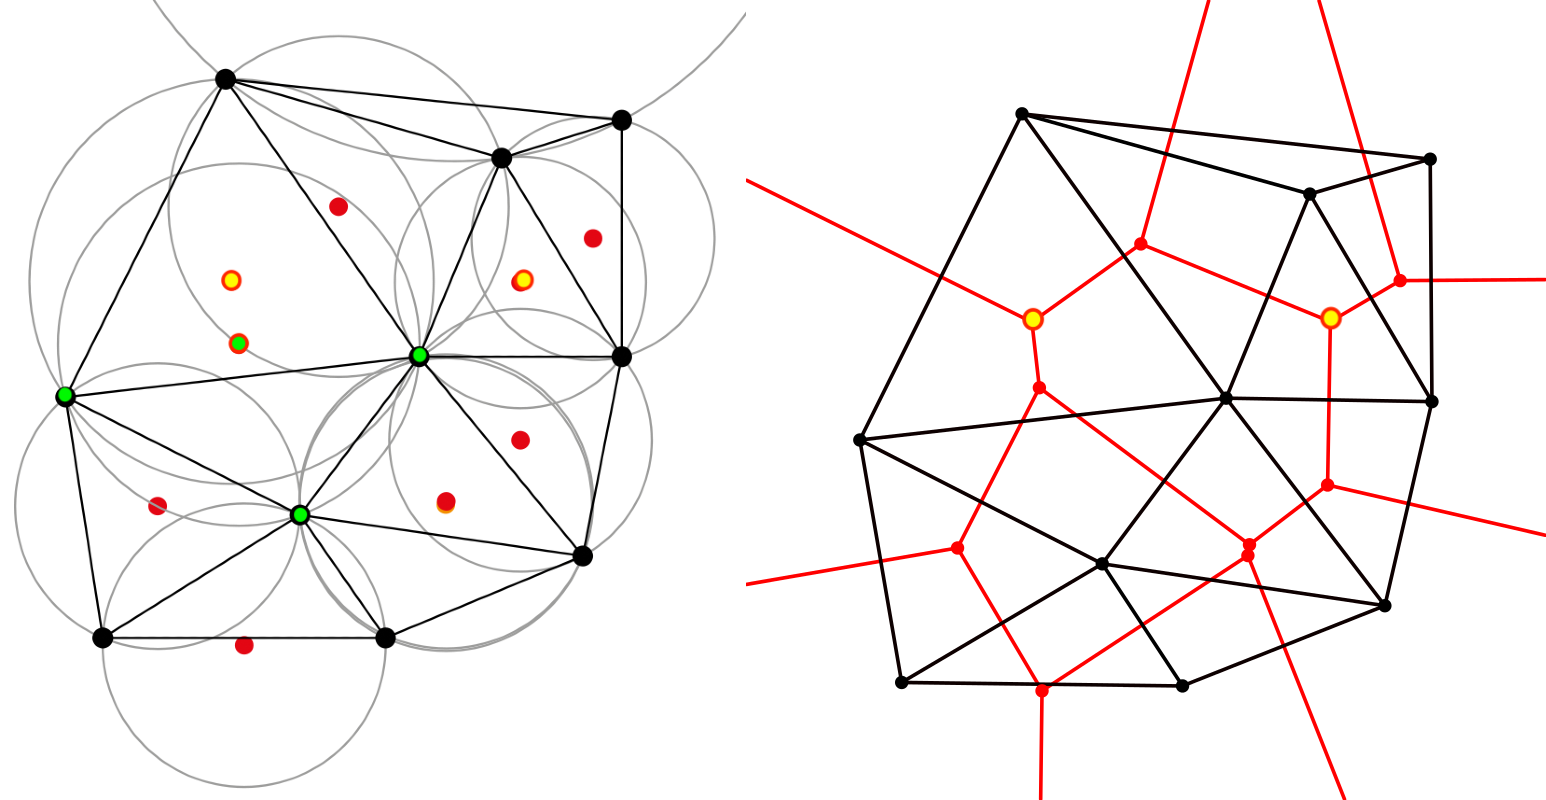
\includegraphics[width=64mm]{content/geometry/Delaunay-Voronoi}}

On left, the Delaunay triangulation with all the circumcircles and their centers (in red).
On right, connecting the centers of the circumcircles produces the Voronoi diagram (in red).

Green highlighted points show that circumcenter can be outside triangle.
Yellow highlighted points show that Voronoi cell edge is present only triangles have shared edge, \textit{not} shared vertex.

\section{Geometric primitives}
	\kactlimport{Point.h}
	\kactlimport{lineDistance.h}
	\kactlimport{SegmentDistance.h}
	\kactlimport{SegmentIntersection.h}
	\kactlimport{lineIntersection.h}
	\kactlimport{sideOf.h}
	\kactlimport{OnSegment.h}
	\kactlimport{linearTransformation.h}
	\kactlimport{LineProjectionReflection.h}
	\kactlimport{Angle.h}

\section{Circles}
	\kactlimport{CircleIntersection.h}
	\kactlimport{CircleTangents.h}
	\kactlimport{CircleLine.h}
	\kactlimport{CirclePolygonIntersection.h}
	\kactlimport{circumcircle.h}
	\kactlimport{MinimumEnclosingCircle.h}
	\kactlimport{convexHullLineIntersection.h}
	\kactlimport{kIntersection.h}

\section{Polygons}
	\kactlimport{InsidePolygon.h}
	\kactlimport{PolygonArea.h}
	\kactlimport{PolygonCenter.h}
	\kactlimport{PolygonCut.h}
	\kactlimport{ConvexHull.h}
	\kactlimport{HullDiameter.h}
	\kactlimport{PointInsideHull.h}
	\kactlimport{LineHullIntersection.h}

\section{Misc. Point Set Problems}
%	\kactlimport{ClosestPair.h}
	\kactlimport{ManhattanMST.h}
	\kactlimport{kdTree.h}
	% \kactlimport{DelaunayTriangulation.h}
	\kactlimport{FastDelaunay.h}
	\kactlimport{VoronoiDiagrams.h}

\section{3D}
	\kactlimport{PolyhedronVolume.h}
	\kactlimport{Point3D.h}
	\kactlimport{3dHull.h}
	\kactlimport{sphericalDistance.h}
